\documentclass[11pt]{article}
\usepackage[margin=1in]{geometry}
\usepackage{booktabs}
\usepackage{graphicx}
\usepackage{hyperref}

\title{CAI6734 Weekly Report 7: Training Collapse Diagnosis and a Full-Pass Baseline}
\author{Omer Kahveci}
\date{November 10, 2026}

\begin{document}
\maketitle

\section{Project Objective}

The Week 6 report left two issues open: the 1.5x test-cost variant had
collapsed during training, and the logs contained repeated invalid-format
warnings after requests for a \texttt{Complete Blood Count (CBC)} action. This
week I set out to find the cause of the collapse, to establish a baseline
trained on the full training split, and to report its results with 95\%
confidence intervals and paired significance tests.

I decided to build a new baseline rather than continue the cost-multiplier
comparison from Week 6. The earlier models were trained on only 300 of the
1,920 training patients, partly on code that was later corrected, and they
saved only aggregate metrics, so they could not support paired comparisons.
Comparing new variants against a weak or inconsistent reference would make any
improvement hard to interpret. The baseline uses the paper's unscaled
test-cost penalty (multiplier 1.0), because it is the paper's method and
therefore the natural reference for every later change.

\section{Accomplishments}

\subsection*{My Contributions This Week}

\begin{itemize}
  \item Diagnosed the training collapse from per-episode logs, which I added to
        the training and evaluation pipeline as planned in Week 6.
  \item Implemented three fixes: test-name matching, a change to the cost
        reward for failed episodes, and an automatic collapse guard.
  \item Ran the full-pass baseline (1,920 training steps with 20 validation
        passes), a zero-shot baseline, and test evaluations of four
        checkpoints on the HiPerGator cluster.
  \item Found and fixed a bug in the Hypothesis Agent's training loss, and
        wrote a unit test that checks the fix against the paper's original
        computation.
  \item Wrote scripts to plot every training and validation metric over time
        and to compute confidence intervals, paired tests, and AUROC.
  \item Began a review of recent literature on reinforcement learning for
        multi-turn agents and sequential diagnosis.
\end{itemize}

\subsection*{Cause of the Training Collapse}

My first attempt at the full-pass baseline collapsed in the same way as the
1.5x variant: 98.6\% of validation episodes were undiagnosed at step 100 and
100\% by step 400. Because the Week 6 logs contained only aggregate metrics, I
first extended the pipeline to record every action of every episode in a CSV
file. These records showed that two problems combined:

\begin{itemize}
  \item \textbf{A test-name mismatch.} The model frequently requested
        \texttt{Complete Blood Count (CBC)}. The environment accepted only the
        exact name \texttt{Complete Blood Count}, so it rejected the request as
        an unknown test (1,407 times in the 1.5x log). The model then often
        replied to the error message in a form that could not be parsed,
        ending the episode. In total, 99\% of the format failures occurred on
        the Decision Agent's second action.
  \item \textbf{Test cost charged to failed episodes.} As in the paper, the
        reward subtracted test costs even from episodes that ended with an
        invalid action. When all four rollouts for a patient failed, the
        rollout that failed before ordering any test therefore received the
        highest reward. GRPO normalizes rewards within each group, so this
        difference became a full-strength signal to fail early.
\end{itemize}

The Week 5 model, which trained with the same reward, appears to have escaped
this trap by learning the format during its first training phase; I have not
verified why that run succeeded.

I made three changes, each targeting one part of the failure:

\begin{itemize}
  \item A listed test name followed by a bracketed abbreviation is now
        accepted as that test. This removes the most common source of error
        messages without accepting test names that are not on the list.
  \item Test cost is no longer charged to invalid episodes, so a group in
        which every rollout fails produces no learning signal instead of a
        signal to fail early. Valid episodes are charged exactly as in the
        paper. This is a deviation from the paper, and I will report it as
        such.
  \item Training stops automatically if at least 95\% of validation episodes
        are undiagnosed at any validation from step 200 onward. A full run
        takes days of GPU time, and the first attempt had already used many
        hours of it before the collapse was noticed.
\end{itemize}

\subsection*{Full-Pass Baseline}

The second attempt trained for 1,920 steps, one pass over every training
patient. I validated on all 240 validation cases every 100 steps rather than
only at the end, so that the learning curve would show when the model
improved or degraded and so that checkpoints could be chosen from validation
results. The model learned the action format quickly: validation accuracy rose
from 3.1\% before training to 42.5\% at step 100. Figure~\ref{fig:validation}
shows the full validation curve: accuracy plateaued from about step 300 and
peaked at step 600, while test cost per case fell steadily toward zero.

\begin{figure}[htbp]
  \centering
  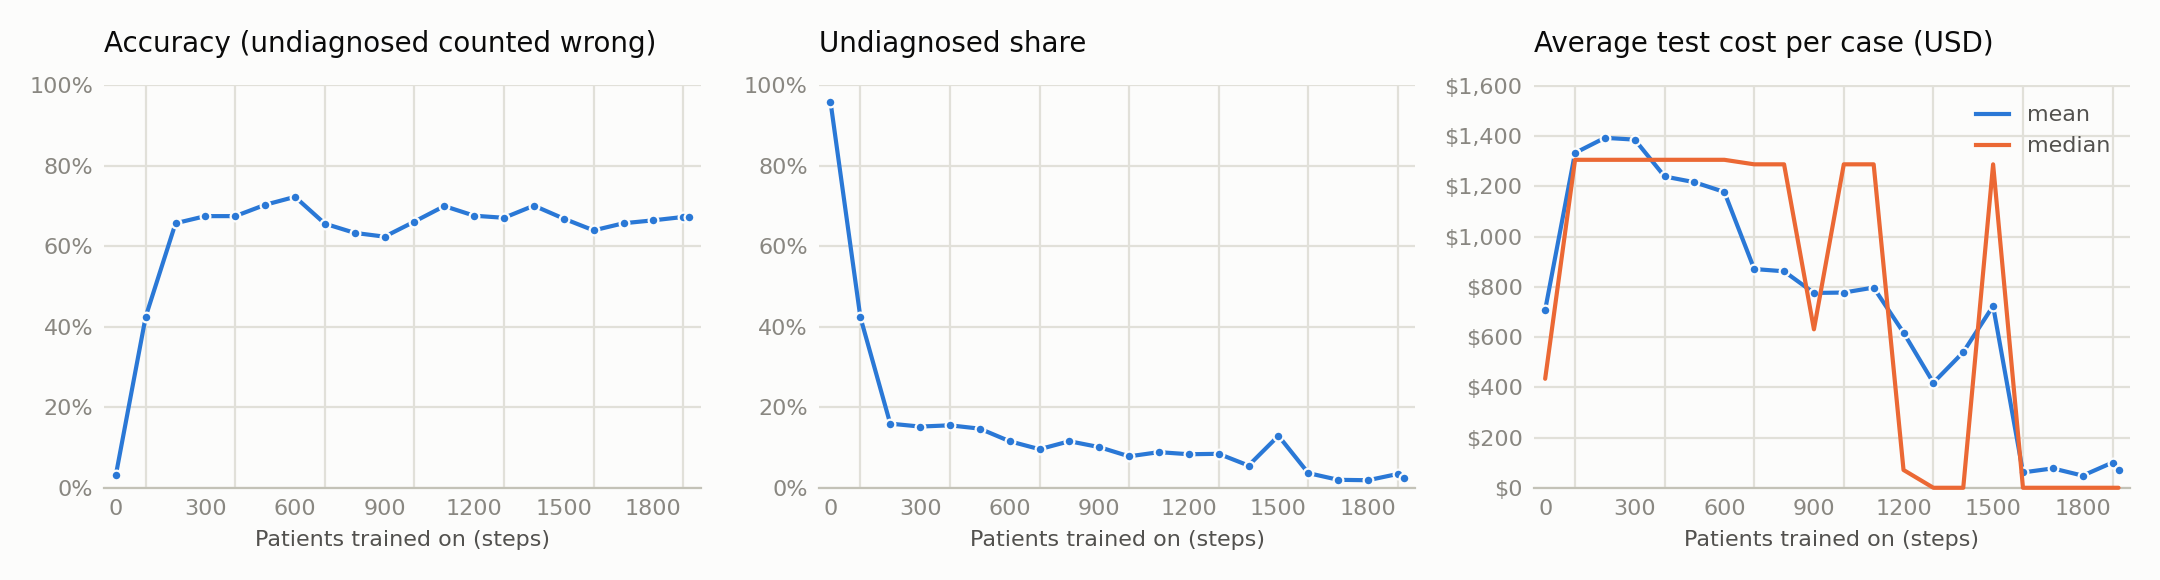
\includegraphics[width=\textwidth]{validation_overview.png}
  \caption{Validation results every 100 training steps (240 cases, four
  sampled rollouts each): accuracy, share of undiagnosed episodes, and test
  cost per case.}
  \label{fig:validation}
\end{figure}

The training schedule alternates three 100-step phases (Decision Agent,
Hypothesis Agent supervised training, and confidence calibration), so a full
cycle is 300 steps, and adapters were saved at the end of each cycle. I chose
step 600 for testing because it had the best validation results, and I made
that choice before seeing any test results; selecting a checkpoint by its test
score would overstate its performance. I also tested steps 300, 1,800, and
1,920 to document how the model changed over training. Step 1,800 is the last
complete cycle; step 1,920 is the final model.

Table~\ref{tab:test} reports test results on the 240-case test split, with one
near-deterministic rollout per case. Intervals are 95\% confidence intervals
(Wilson for accuracy, patient-level bootstrap with 5,000 resamples otherwise).

\begin{table}[ht]
  \centering
  \caption{Test results (240 cases). Class-mean accuracy is the mean of the
  four per-disease accuracies.}
  \label{tab:test}
  \small
  \begin{tabular}{lrrrrr}
    \toprule
    Metric & Zero-shot & Step 300 & Step 600 & Step 1,800 & Step 1,920 \\
    \midrule
    Accuracy & 8.8\% & 75.8\% & \textbf{85.4\%} & 66.7\% & 70.8\% \\
    \quad 95\% CI & [5.8, 13.0] & [70.0, 80.8] & [80.4, 89.3] & [60.5, 72.3] & [64.8, 76.2] \\
    Class-mean accuracy & 9.0\% & 72.7\% & \textbf{84.3\%} & 63.7\% & 65.2\% \\
    Macro F1 & 15.5\% & 71.9\% & \textbf{84.0\%} & 62.3\% & 65.4\% \\
    Undiagnosed & 87.9\% & 2.5\% & 2.1\% & 0.0\% & 0.0\% \\
    Tests per case & 1.16 & 1.62 & 1.19 & 0.00 & 0.00 \\
    Cost per case & \$798 & \$1,435 & \$1,259 & \$0 & \$0 \\
    Calibration error (ECE) & 10.9\% & 12.0\% & 14.8\% & 31.7\% & 28.4\% \\
    AUROC, confidence vs.\ correct & 0.784 & 0.728 & 0.750 & 0.500 & 0.506 \\
    \bottomrule
  \end{tabular}
\end{table}

Because every model was evaluated on the same 240 patients, I used paired
tests, which compare the models patient by patient and are more sensitive than
comparing two overall accuracies. Table~\ref{tab:paired} compares step 600
with the other checkpoints, using an exact McNemar test for accuracy and paired
permutation tests for the other metrics. All differences shown remain
significant after Holm correction for multiple comparisons.

\begin{table}[ht]
  \centering
  \caption{Step 600 minus each other checkpoint, on the same 240 patients.}
  \label{tab:paired}
  \small
  \begin{tabular}{lrrrr}
    \toprule
    Compared with & Accuracy [95\% CI] & $p$ & Macro F1 & Cost per case \\
    \midrule
    Zero-shot & +76.7 [+71.2, +81.7] & $<0.001$ & +68.4 & +\$461 \\
    Step 300 & +9.6 [+4.6, +14.6] & $<0.001$ & +12.1 & $-$\$176 \\
    Step 1,800 & +18.8 [+12.1, +25.4] & $<0.001$ & +21.7 & +\$1,259 \\
    Step 1,920 & +14.6 [+8.3, +20.8] & $<0.001$ & +18.6 & +\$1,259 \\
    \bottomrule
  \end{tabular}
\end{table}

The step-600 model is significantly more accurate than the step-300 model and
also cheaper. The paper reports 81.3\% class-mean accuracy, 81.3\% macro F1,
and \$1,295.61 mean cost for LA-CDM with the cost reward. All three values lie
inside the step-600 confidence intervals, so the reproduction matches the
paper's results; it does not demonstrate an improvement over them. The
comparison is indicative only, because the paper's test split differs from
ours. Figure~\ref{fig:cost} places each checkpoint and the paper's result on
the trade-off between cost and accuracy.

\begin{figure}[htbp]
  \centering
  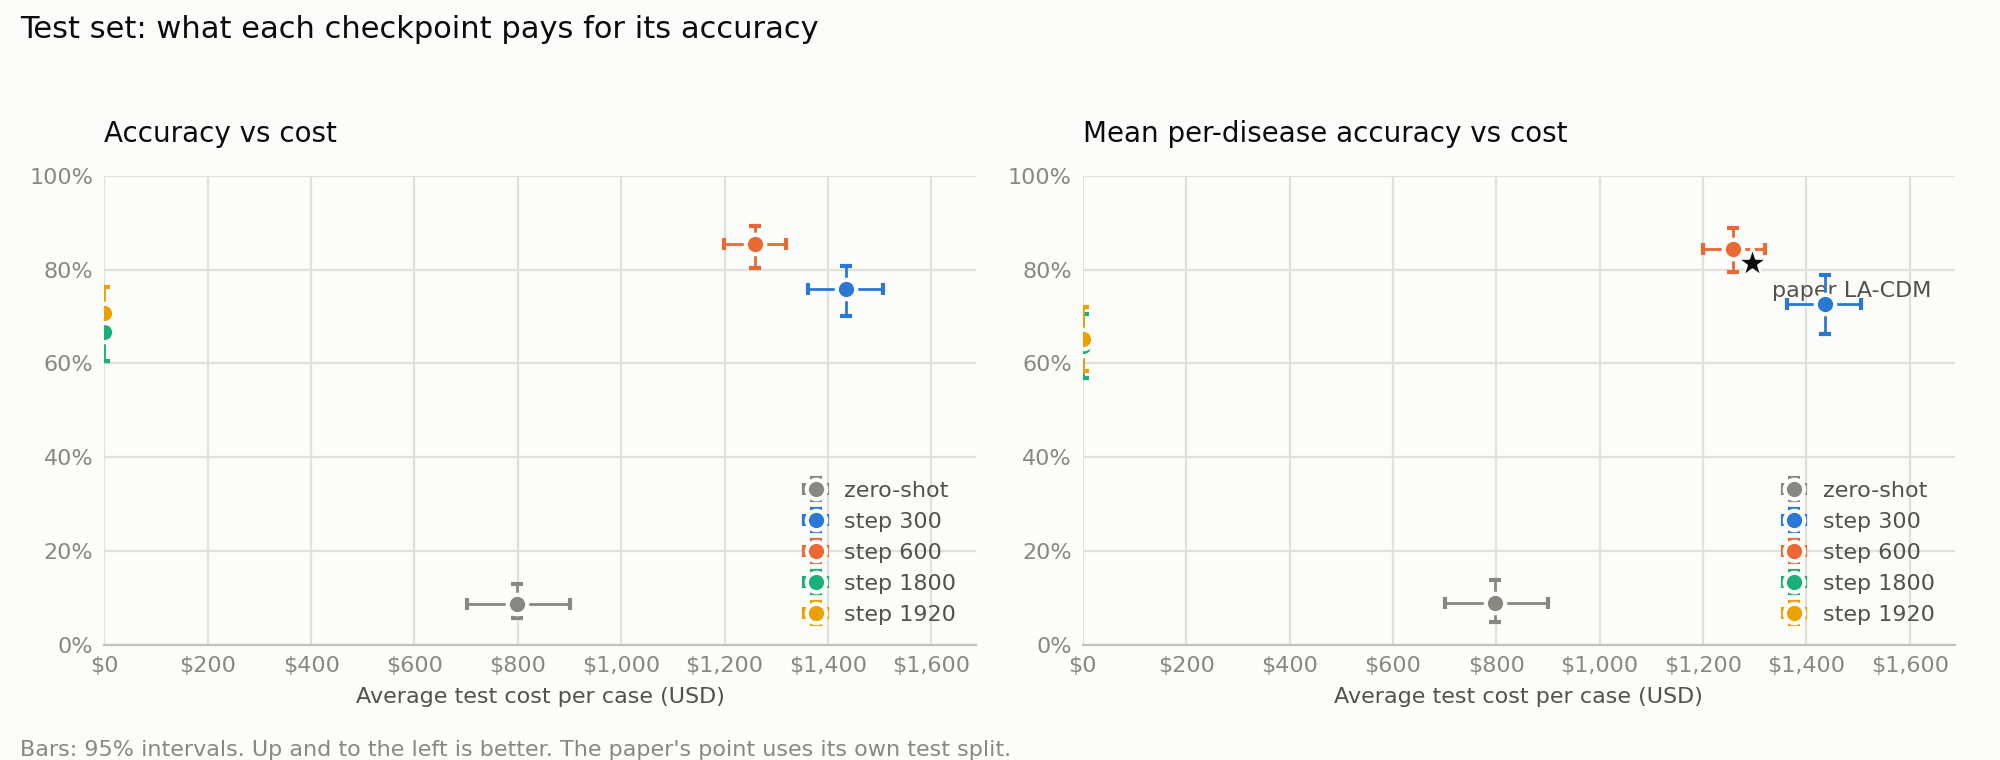
\includegraphics[width=0.75\textwidth]{test_cost_vs_accuracy.png}
  \caption{Test accuracy against mean test cost per case for each checkpoint,
  with the paper's LA-CDM result for reference.}
  \label{fig:cost}
\end{figure}

Test accuracy is about 13 points higher than validation accuracy at the same
step (72.3\%). The main reason is the evaluation protocol: validation samples
four rollouts per case at temperature 0.9 with shorter token limits, whereas
the test evaluation uses one near-deterministic rollout. The same gap appears
before training (3.1\% validation versus 8.8\% zero-shot test accuracy). I
therefore use validation only to compare checkpoints with one another, and the
test set to compare with the paper.

\subsection*{Findings from the Long Run}

\begin{itemize}
  \item \textbf{The Decision Agent drifts toward ordering no tests.} Tests per
        validation case fell from 1.68 at step 100 to about 0.05 by step
        1,600, and the step-1,800 and step-1,920 models ordered no tests at
        all on the test set. Once the four rollouts for a patient agree on the
        diagnosis, test cost is the only remaining difference in reward, so
        training keeps pushing toward fewer tests. These two checkpoints still
        reached 67--71\% accuracy from the patient history alone, which
        suggests that the tests contribute about 15 points of accuracy at
        step 600.
  \item \textbf{Hypothesis Agent calibration does not improve.} The trained
        model's confidence separates right from wrong diagnoses no better than
        the untrained model's (AUROC 0.750 versus 0.784), and its calibration
        error rises over training. After step 600 the confidence carries no
        information (AUROC 0.50). A likely cause is that both agents share a
        single LoRA adapter, so updates for one agent shift the other's
        confidence outputs; this has not been verified.
  \item \textbf{Pancreatitis remains the weakest class.} Its recall stayed at
        61--67\% at every trained checkpoint, while the other three diseases
        improved substantially. At step 600, 13 of 54 pancreatitis cases were
        diagnosed as cholecystitis (Figure~\ref{fig:confusion}).
\end{itemize}

\begin{figure}[htbp]
  \centering
  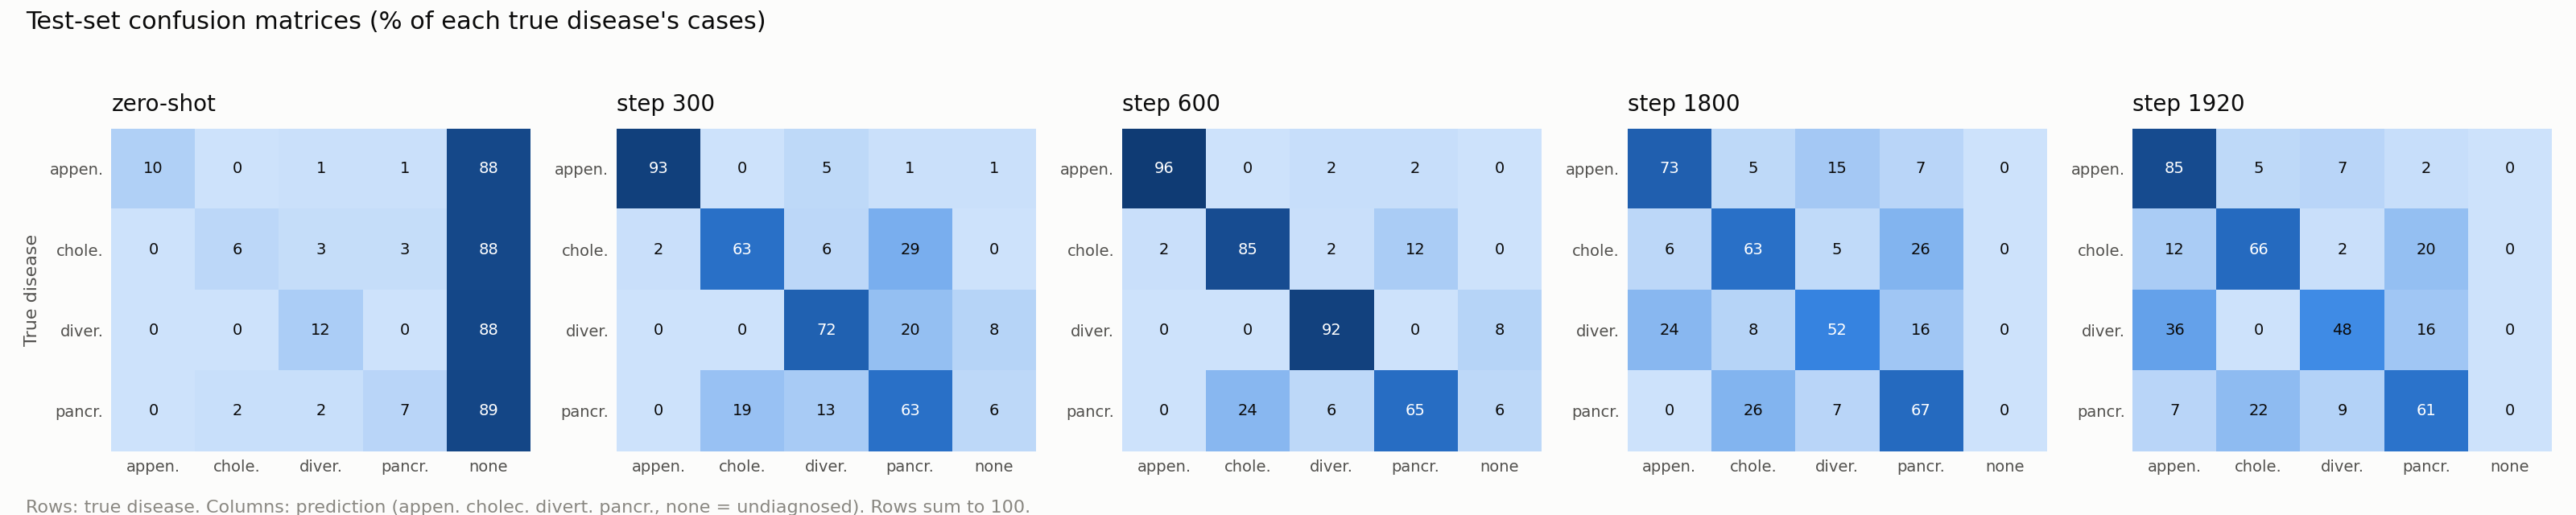
\includegraphics[width=\textwidth]{test_confusion.png}
  \caption{Test confusion matrices for each checkpoint. Rows are the true
  disease and columns the model's diagnosis.}
  \label{fig:confusion}
\end{figure}

\subsection*{Hypothesis Agent Training Bug}

While reviewing why the Hypothesis Agent's accuracy barely changed during
training, I found a bug in its supervised training loss, introduced in an
optimization made in late September. The loss scored only the final positions
of each padded sequence, assuming that the answer occupied those positions.
Because the sequences are padded on the right, this held only for the longest
sequence in each batch; every shorter sequence contributed no loss. In effect,
each step trained the Hypothesis Agent on a single prompt at reduced strength.
The bug affected every training run since September, including the Week 5 and
Week 6 models and the baseline above, but not evaluation.

I fixed the loss and wrote a unit test confirming that it equals the
computation in the paper's original code on a small model. I then started a
third baseline run that differs from the second only by this fix. Changing
nothing else means that any difference between the two runs can be attributed
to the fix.

\subsection*{What I Learned}

With a sparse reward and only four rollouts per patient, small reward
differences that do not reflect diagnostic quality, such as the test cost of a
failed episode, can dominate GRPO's learning signal; how a reward treats
failed episodes matters as much as how it treats successful ones. Longer
training is not better under the paper's cost reward: accuracy peaked at step
600 and declined as the Decision Agent stopped ordering tests, so the choice
of checkpoint mattered more than the length of the run. Finally, the trained
Hypothesis Agent became more accurate without becoming better at knowing when
it is right, which matters because the decision to stop ordering tests depends
on that judgment.

\section{Challenges}

The step-600 result was obtained with the Hypothesis Agent bug present, so the
effect of the fix is not yet known. The run is also a single training run:
the confidence intervals cover sampling of test cases but not training
randomness. The diverticulitis class has only 25 test cases, so its
per-disease intervals span 20--40 points. The AUROC across the four diseases
could only be approximated, because the logs keep one hypothesis and one
confidence per turn rather than a probability for each disease. Finally,
training is slow: each 100-step block, including its validation pass, takes
several hours on the available GPUs, so the full run took more than two days.

\section{Next Steps}

The findings above show that the main remaining weaknesses lie in the agentic
search itself: how the Decision Agent decides which tests to order and when to
stop, and how reliably the Hypothesis Agent's confidence guides that decision.
Next week I will:

\begin{itemize}
  \item Review state-of-the-art literature on agentic search, particularly
        reinforcement learning for multi-turn, information-seeking agents and
        sequential clinical diagnosis, to identify changes to the agentic loop
        that address these weaknesses. Initial candidates include rewarding
        each test by how much it increases the probability of the correct
        diagnosis (IGPO, ICLR 2026), stopping once the diagnostic agent is
        confident enough (LDTL, 2026, evaluated on the same MIMIC-CDM
        benchmark), and rewards that penalize both stopping too early and
        searching too much. I will select the most promising change based on
        how directly it targets these failures and how much implementation
        and GPU time it requires.
  \item Finish the third baseline run with the Hypothesis Agent fix and compare
        it with the second run at matched steps, so that the selected
        improvement is evaluated against the corrected baseline.
\end{itemize}

Improving Hypothesis Agent calibration and resuming the test-cost multiplier
comparison from Week 6 are planned after these steps, because both depend on
the corrected baseline.

\section{AI Disclaimer}

I used OpenAI Codex and Anthropic Claude to assist with implementing the
experiment, inspecting training and evaluation logs, computing the statistics,
and drafting this report.

\end{document}
